\documentclass[12pt,border=5pt]{standalone}

\usepackage{tikz}
\usetikzlibrary{arrows.meta}

\begin{document}
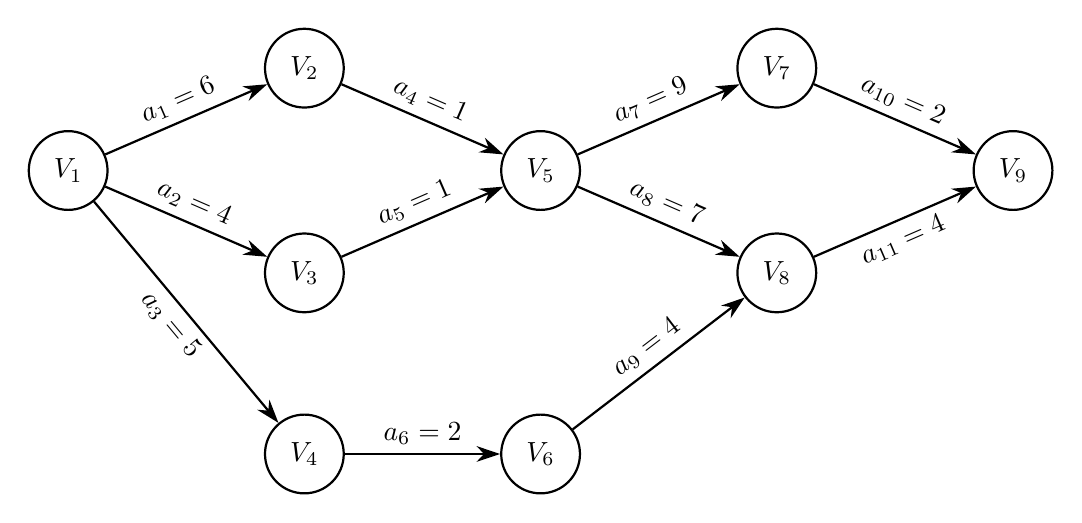
\begin{tikzpicture}[
    thick,
    >={Stealth[length=3mm,width=2mm]},
    event/.style={circle,draw,minimum size=10mm,inner sep=0pt},
    activity/.style={midway,sloped,above,inner sep=3pt}
]
    \node[event] (v1) at (0,0) {$V_1$};
    \node[event] (v2) at (3,1.3) {$V_2$};
    \node[event] (v3) at (3,-1.3) {$V_3$};
    \node[event] (v4) at (3,-3.6) {$V_4$};
    \node[event] (v5) at (6,0) {$V_5$};
    \node[event] (v6) at (6,-3.6) {$V_6$};
    \node[event] (v7) at (9,1.3) {$V_7$};
    \node[event] (v8) at (9,-1.3) {$V_8$};
    \node[event] (v9) at (12,0) {$V_9$};

    \draw[->] (v1) -- node[activity] {$a_1=6$} (v2);
    \draw[->] (v1) -- node[activity] {$a_2=4$} (v3);
    \draw[->] (v1) -- node[activity,below] {$a_3=5$} (v4);
    \draw[->] (v2) -- node[activity] {$a_4=1$} (v5);
    \draw[->] (v3) -- node[activity] {$a_5=1$} (v5);
    \draw[->] (v4) -- node[activity] {$a_6=2$} (v6);
    \draw[->] (v5) -- node[activity] {$a_7=9$} (v7);
    \draw[->] (v5) -- node[activity] {$a_8=7$} (v8);
    \draw[->] (v6) -- node[activity] {$a_9=4$} (v8);
    \draw[->] (v7) -- node[activity] {$a_{10}=2$} (v9);
    \draw[->] (v8) -- node[activity,below] {$a_{11}=4$} (v9);
\end{tikzpicture}
\end{document}
